% 2016 공주대 워크숍
% 텍 매크로 작성법

\documentclass{beamer}

\usetheme{metropolis}
\metroset{inner/sectionpage=none}
\metroset{outer/progressbar=head}
\metroset{color/block=fill}

\usepackage{kotex}

\hypersetup{pdfencoding=auto}


% title
\title{텍 매크로 작성법}
\subtitle{텍 매크로 작성의 기초와 응용}
\author{남수진}
\date{2016년 11월 5일(토)}
\institute{
  2016 공주대학교 문서작성 워크숍 2016\\
  공주대학교 인문사회과학관 1층 컴퓨터실 107호}


%%
\begin{document}

\maketitle


%
\begin{frame}{매크로 관련 명령어}
  \vspace{4mm}
  \hbox to\hsize{\hss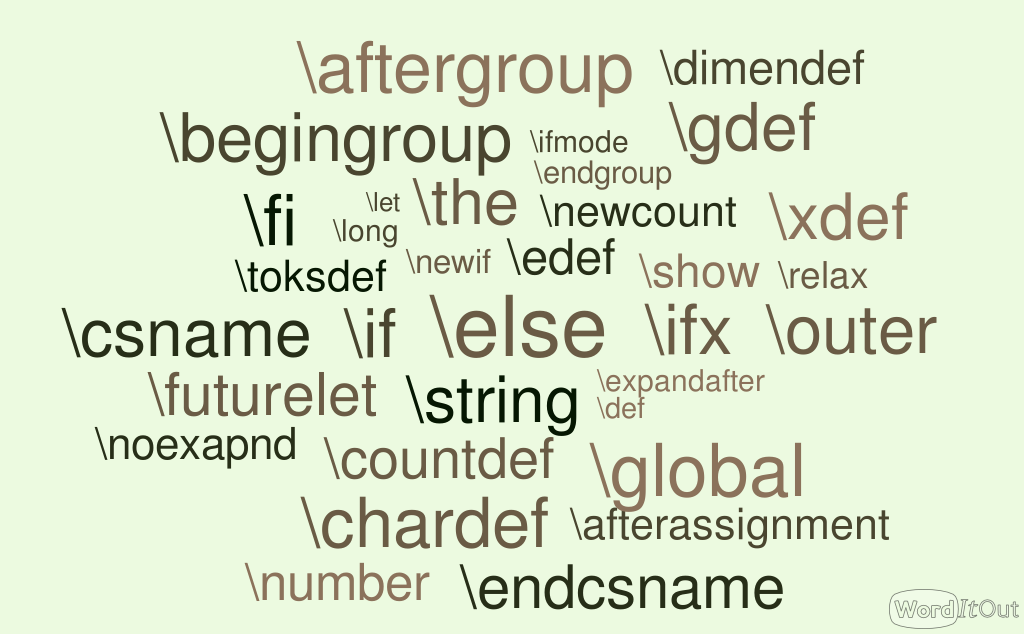
\includegraphics[height=7.5cm]{cs.png}\hss}
\end{frame}


%
\begin{frame}[fragile]{매크로}
  The \TeX\ Hierarchy, TUGboat, Volume 15 (1994), No.1, 7---9.
  \begin{description}
  \item [Novice] has heard of macros, but has never seen one.
  \item [User] writes macros that are used once, and that are
    longer than the code they replace.
  \item [Programmer], having been bitten by unwanted spaces,
    writes macros that don't contain spaces, and every line ends with
    a `{\small\verb+%+}'.
  \item [Hacker] has written self-modifying macros, writes
    {\small\verb+\endlinechar=-1+} or {\small\verb+\catcode'\^^M=9+}
    to prevent having to put {\small\verb+%+}'s at the end of lines in macros.
  \item [Guru] has written macros containing {\small\verb+####+}, more than 3
    {\small\verb+\expandafter+}'s in a row, and the sequence
    {\small\verb+\expandafter\endcsname+}.
  \end{description}
\end{frame}


%
\begin{frame}[fragile]{매크로 정의}
  \begin{itemize}
  \item 문서에서 여러번 반복적으로 사용되는 문구나 명령어의 나열을 하나의 명령어로 만든 것
    
    \medskip
    \hbox to\hsize{\hss
      \verb+\def+<control sequence><parameter text>%
      \verb+{+<replacement text>\verb+}+\hss}
    \medskip
  \item 텍의 전개 과정에서 매크로는 치환문으로 교체된다.
  \item 텍은 입력(input, eyes), 전개(expansion, mouth),
    실행(execution, stomach), 출력(visual, bowels)의 과정을 거친다.
  \end{itemize}
\end{frame}


%
\begin{frame}[fragile]{\texttt{BOLD} 매크로 만들기}
  \begin{verbatim}
    {\bf Hello world}
    
    \BOLD{Hello world}
  \end{verbatim}
  \begin{alertblock}{Programmer}
    \verb+\def\BOLD#1{{\bf #1}}+
  \end{alertblock}
\end{frame}


%
\begin{frame}[fragile]{\texttt{BOLD} 매크로 만들기}
  \begin{verbatim}
    \BOLD{
      Hello

      world
    }

    Runaway argument?
    { Hello
    ! Paragraph ended before \BOLD was complete.
  \end{verbatim}
  \begin{alertblock}{Programmer first class}
    \verb+\long\def\BOLD#1{{\bf #1}}+
  \end{alertblock}
\end{frame}


%
\begin{frame}[fragile]{\texttt{BOLD} 매크로 만들기}
  \begin{alertblock}{Hacker}
    \verb+\def\beginbold{\bgroup\bf}+
    
    \verb+\def\endbold{\egroup}+
  \end{alertblock}

  \begin{verbatim}
    \beginbold
    Hello

    world
    \endbold
  \end{verbatim}
\end{frame}


%
\begin{frame}[fragile]{\texttt{BOLD} 매크로 만들기}
  \begin{alertblock}{Wizard}
    \verb+\def\BOLD{\bgroup\bf\let\next=}+
  \end{alertblock}
  \medskip
  \begin{exampleblock}{Guru}
    \verb+\def\BOLD#{\bgroup\bf\let\next= }+
  \end{exampleblock}
\end{frame}


%
\begin{frame}{관련문서}
  \begin{itemize}
  \item \url{https://github.com/sjnam/TeX/2016-workshop}
  \item \href{http://ftp.ktug.org/tex-archive/systems/knuth/dist/tex/}
    {The \TeX book}
  \item \href{http://ftp.ktug.org/tex-archive/info/impatient/book.pdf}
    {\TeX\ fot the Impatient}
  \item \href{http://ftp.ktug.org/tex-archive/info/texbytopic/TeXbyTopic.pdf}
    {\TeX\ By Topic}
  \item \href{https://www.tug.org/TUGboat/tb14-1/tb38laan.pdf}
    {FIFO and LIFO sing the BLUes}
  \item \href{https://www.tug.org/TUGboat/tb08-3/tb19knut.pdf}
    {Macros for Jill}
  \item \href{https://www.tug.org/TUGboat/tb15-1/tb42arseneau.pdf}
    {The TeX\ Hierarchy}
  \end{itemize}
\end{frame}


%
\plain{\huge ¿Tienes alguna pregunta?}


\end{document}
